% fs-13-anova.tex

\documentclass[xcolor=dvipsnames]{beamer}
\usepackage{teachbeamer}

\title{ANOVA}
\subtitle{{\CourseNumber}, BCIT}

\author{\CourseName}

\date{May 7, 2018}

% \begin{figure}[h]
% 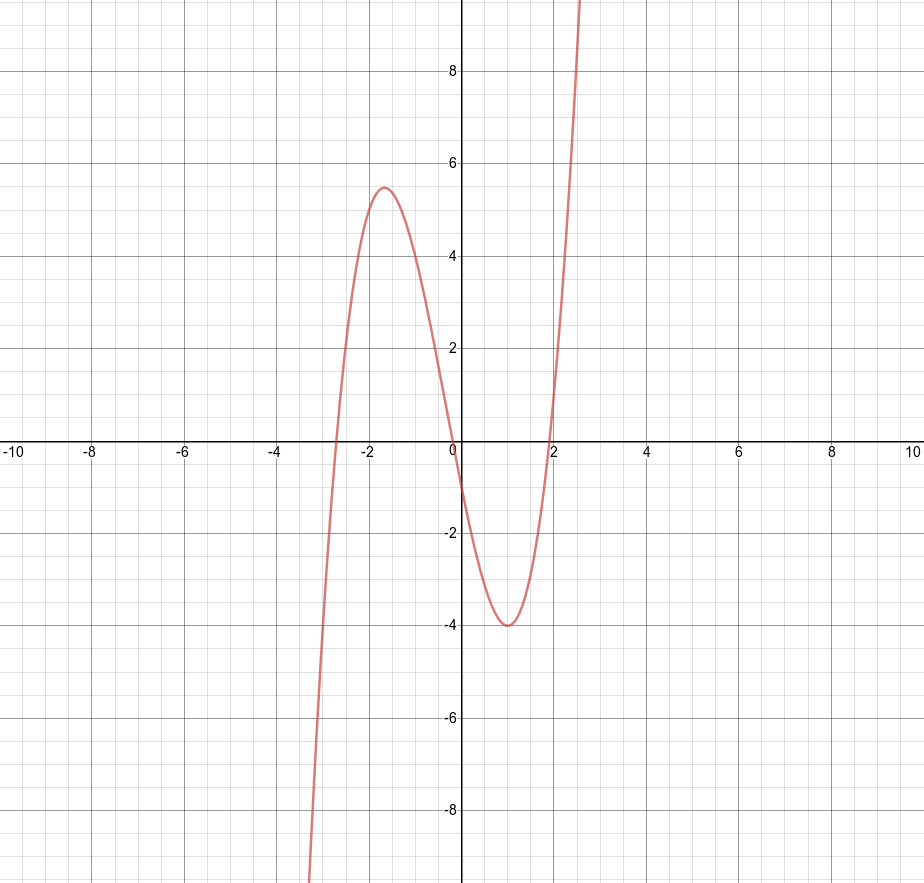
\includegraphics[scale=.3]{./diagrams/extrema1.png}
% \end{figure}

% Command             10pt    11pt    12pt
% \tiny               5       6       6
% \scriptsize         7       8       8
% \footnotesize       8       9       10
% \small              9       10      10.95
% \normalsize         10      10.95   12

\begin{document}

\begin{frame}
  \titlepage
\end{frame}

\begin{frame}
  \frametitle{Analysis of Variance}
One-way analysis of variance (ANOVA) is a method of testing the
equality of three or more population means by analyzing sample
variances. One-way analysis of variance is used with data categorized
with one factor (or treatment), so there is one characteristic used to
separate the sample data into the different categories.

\bigskip

Consider the R Statistics code on the following page. It corresponds
to the narrative in Triola, page 562. The result is a test statistic
following the $F$-distribution and a $p$-value that can be compared to
the significance level. This type of ANOVA is always a right-hand
one-tailed test.
% http://pages.stat.wisc.edu/~yandell/st571/R/anova.pdf
\end{frame}

\begin{frame}[fragile]
  \frametitle{Analysis of Variance}
\begin{scriptsize}
\begin{alltt}
l<-c(85,90,107,85,100,97,101,64,111,100,76,136,100,90,135,104,149,99,1
  07,99,113,104,101,111,118,99,122,87,118,113,128,121,111,104,51,100,113,
  82,146,107,83,108,93,114,113,94,106,92,79,129,114,99,110,90,85,94,127,
  101,99,113,80,115,85,112,112,92,97,97,91,105,84,95,108,118,86,89,100)
m<-c(78,97,107,80,90,83,101,121,108,100,110,111,97,51,94,80,101,92,100,
  77,108,85)
h<-c(93,100,97,79,97,71,111,99,85,99,97,111,104,93,90,107,108,78,95,78,
  86)
n<-c(length(l),length(m),length(h))
group<-rep(1:3,n)
y<-c(l,m,h)
data<-data.frame(y=y,group=factor(group))
fit<-lm(y~group,data)
anova(fit)
\end{alltt}
\end{scriptsize}
\end{frame}

\begin{frame}
  \frametitle{Anova: Lead and Intelligence Quotients (low)}
  \begin{figure}[h]
    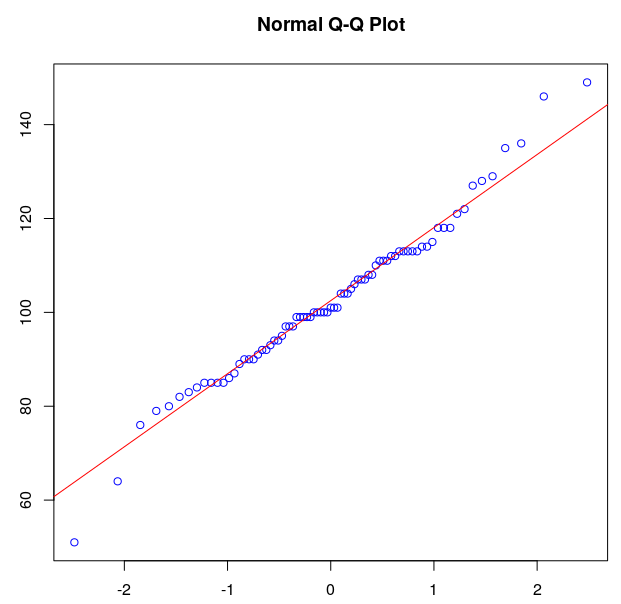
\includegraphics[scale=0.35]{./diagrams/lead_l.png}
  \end{figure}
\end{frame}

\begin{frame}
  \frametitle{Anova: Lead and Intelligence Quotients (medium)}
  \begin{figure}[h]
    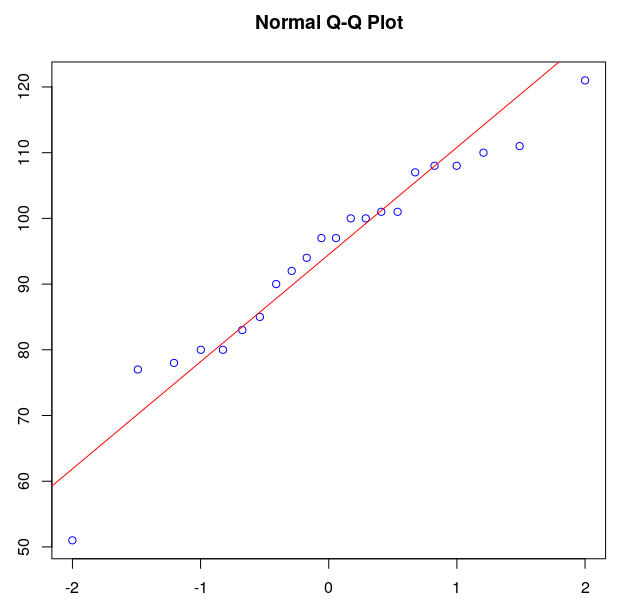
\includegraphics[scale=0.35]{./diagrams/lead_m.png}
  \end{figure}
\end{frame}

\begin{frame}
  \frametitle{Anova: Lead and Intelligence Quotients (high)}
  \begin{figure}[h]
    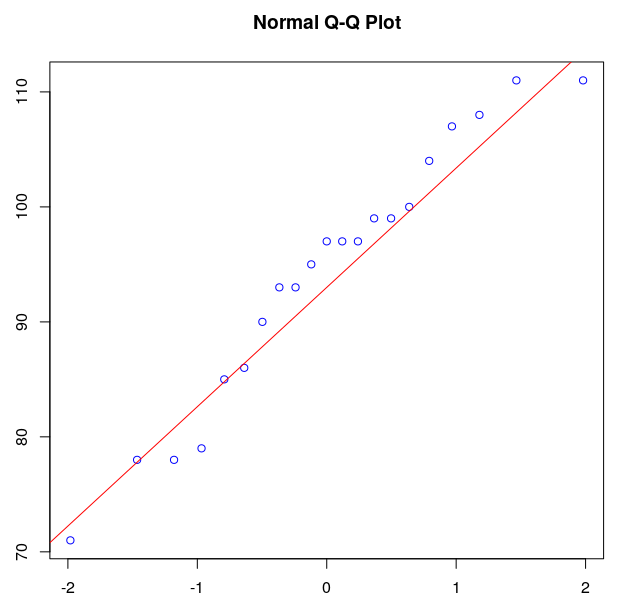
\includegraphics[scale=0.35]{./diagrams/lead_h.png}
  \end{figure}
\end{frame}

\begin{frame}
  \frametitle{Anova: Lead and Intelligence Quotients (boxplots)}
\begin{figure}[h]
  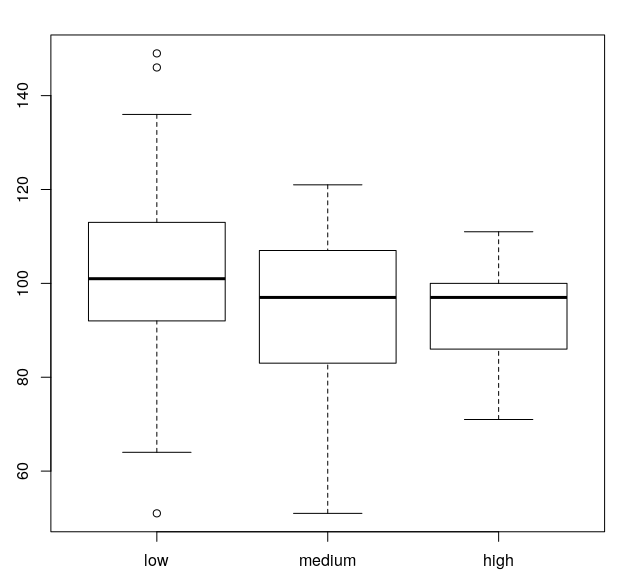
\includegraphics[scale=0.35]{./diagrams/lead_bp.png}
\end{figure}
\end{frame}

\begin{frame}[fragile]
  \frametitle{Anova: Lead and Intelligence Quotients}
  R Statistics yields the following output:
\begin{verbatim}
Analysis of Variance Table

Response: y
           Df  Sum Sq Mean Sq F value Pr(>F)  
group       2  1920.9  960.45  3.8646 0.0237 *
Residuals 117 29077.1  248.52                 
---
Signif. codes:  0 ‘***’ 0.001 ‘**’ 0.01 ‘*’ 0.05 ‘.’ 0.1 ‘ ’ 1
\end{verbatim}
What is important to us is the test statistic, whose distribution is
the $F$-distribution, $3.8646$; and the $p$-value $0.0237$. Since
ANOVA is always one-tailed, area to the right, all you need to do is
compare the $p$-value to the significance level. ``If $p$ is low, the
NULL must go.''
\end{frame}

\begin{frame}
  \frametitle{$F$-Distribution}
  The $F$-distribution depends on two different degrees of freedom,
  which makes using a table of critical values awkward. We will use
  $p$-values provided by technology instead. A
  table with critical values is here: {\footnotesize
    \texttt{http://www.itl.nist.gov/div898/handbook/eda/section3/eda3673.htm}}.
  The shape of the $F$-distribution is similar to the shape of the
  $\chi^{2}$-distribution.
\begin{figure}[h]
  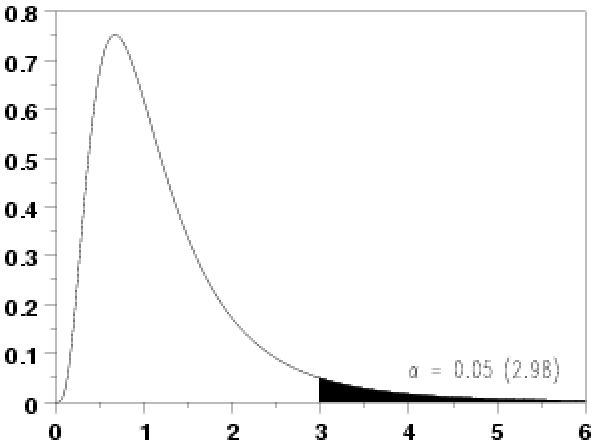
\includegraphics[scale=0.25]{./diagrams/fdist.png}
\end{figure}
\end{frame}

\begin{frame}
  \frametitle{One-Way ANOVA in Microsoft Excel}
For instructions, see {\tiny \texttt{http://www.excel-easy.com/examples/anova.html}}.
  \begin{figure}[h]
    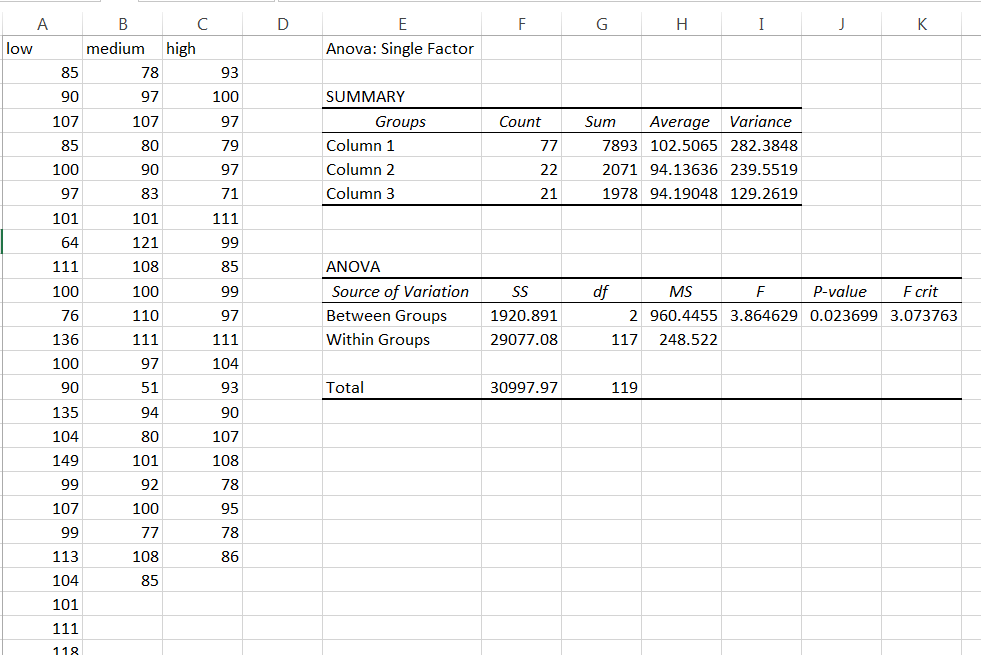
\includegraphics[scale=0.5]{./diagrams/lead-with-anova.png}
  \end{figure}
\end{frame}

\begin{frame}[fragile]
  \frametitle{ANOVA Exercise}
  Susan predicts that students will learn most effectively with a
  constant background sound, as opposed to an unpredictable sound
  or no sound at all. She randomly divides twenty-four students
  into three groups of eight. All students study a passage of text
  for 30 minutes. Those in group 1 study with background sound at
  a constant volume in the background. Those in group 2 study with
  noise that changes volume periodically. Those in group 3 study
  with no sound at all. After studying, all students take a 10
  point multiple choice test over the material. Test the
  appropriate null hypothesis using one-way ANOVA at a 0.05
  significance level.

\begin{footnotesize}
\begin{verbatim}
+----------------+---+---+---+---+---+---+---+---+
| constant sound | 7 | 4 | 6 | 8 | 6 | 6 | 2 | 9 |
+----------------+---+---+---+---+---+---+---+---+
| random sound   | 5 | 5 | 3 | 4 | 4 | 7 | 2 | 2 |
+----------------+---+---+---+---+---+---+---+---+
| no sound       | 2 | 4 | 7 | 1 | 2 | 1 | 5 | 5 |
+----------------+---+---+---+---+---+---+---+---+
\end{verbatim}
\end{footnotesize}
\end{frame}

\begin{frame}
  \frametitle{Final Exam Practice}
  {\ubung} At a gas station, 40\% of customers fill their tanks. Of
  those who fill their tanks, 80\% pay with a credit card.
  \begin{enumerate}
  \item What is the probability that a customer fills their tank and
    pays with a credit card?
  \item What is the probability that either three or four out of ten
    customers fill their tank and pay by credit card?
  \item What is the probability that more than half of eight customers
    fill their tank and pay by credit card?
  \end{enumerate}
\end{frame}

\begin{frame}
  \frametitle{Final Exam Practice}
  {\ubung} At a certain time in the afternoon, London Heathrow sees on average 2
  planes landing per minute.
  \begin{enumerate}
  \item What is the probability of four or more planes landing in one
    minute?
  \item What is the probability that no plane will land in a
    particular minute?
  \end{enumerate}
\end{frame}

\begin{frame}
  \frametitle{End of Lesson}
Next Lesson: End of Term! Have a Happy Holiday!
\end{frame}

\end{document}

